



\documentclass{article}

% The preceding line is only needed to identify funding in the first footnote. If that is unneeded, please comment it out.
\usepackage{cite}
\usepackage{amsmath,amssymb,amsfonts}
\usepackage{algorithmic}
\usepackage{graphicx}
\usepackage{textcomp}
\usepackage{xcolor}
\usepackage{placeins}
\usepackage{hyperref}
\usepackage {graphicx}
\usepackage{multicol}
\usepackage{geometry}
\usepackage{caption}
\usepackage{subcaption}
\usepackage{tikz}
\usepackage{enumitem}
\def\BibTeX{{\rm B\kern-.05em{\sc i\kern-.025em b}\kern-.08em
    T\kern-.1667em\lower.7ex\hbox{E}\kern-.125emX}}
\begin{document}

\makeatletter
\newcommand{\linebreakand}{% required for correct name alignement beyond the third
      \end{@IEEEauthorhalign}
      \hfill\mbox{}\par
      \mbox{}\hfill\begin{@IEEEauthorhalign}
    }
\makeatother

% ======== TITLE SECTION ========
\title{ Exercise 2: Visualizing Neural Networks\\
Advanced Data Analysis and Machine Learning }

% ======== AUTHOR LIST IN ALPHABETICAL ORDER ========
\author{
%\IEEEauthorblockN{Alessio Pagoncelli}
% \IEEEauthorblockA{\textit{MSc/BSc} \\
% \textit{Univeristy}\\
% Location \\
% mail}\and
Janis Waser
% \IEEEauthorblockA{\textit{MSc/BSc} \\
% \textit{Univeristy}\\
% Location \\
% mail}
}
\maketitle

% ======= ABSTRACT AND KEYWORDS ========
%\begin{abstract}
%ABSTRACT TEXT HERE
%\end{abstract}
%
%\begin{IEEEkeywords}
%KEYWORDS
%\end{IEEEkeywords}

% ========================================
% ======== BEGINNING OF MAIN TEXT ========
% ========================================
\section{Neural network}
The utilized neural network consists of only two hidden layers with 80 respectively 60 neurons with Sigmoid as activation functions. The accuracy on the handwritten digits dataset is about 97\%. The script stems from Langelaar (\cite{script}). 

The full code and the used script to create the visualisations can be found on the Github repository (\url{https://github.com/us-ja/ADAML_Homeworks.git}{})
\section{PCA}
It can be observed in Figure \ref{fig:PCA} that the data is somewhat separable already for input layer. The trained neural network improves this separability and for the final layer we can see the data the data is separated in nearly orthogonal structures, which requires more than 2 dimensions since we also have 10 different categories into which we try to classify. 
\begin{figure}[h!]
     \centering
     \begin{subfigure}[b]{0.32\textwidth}
         \centering
         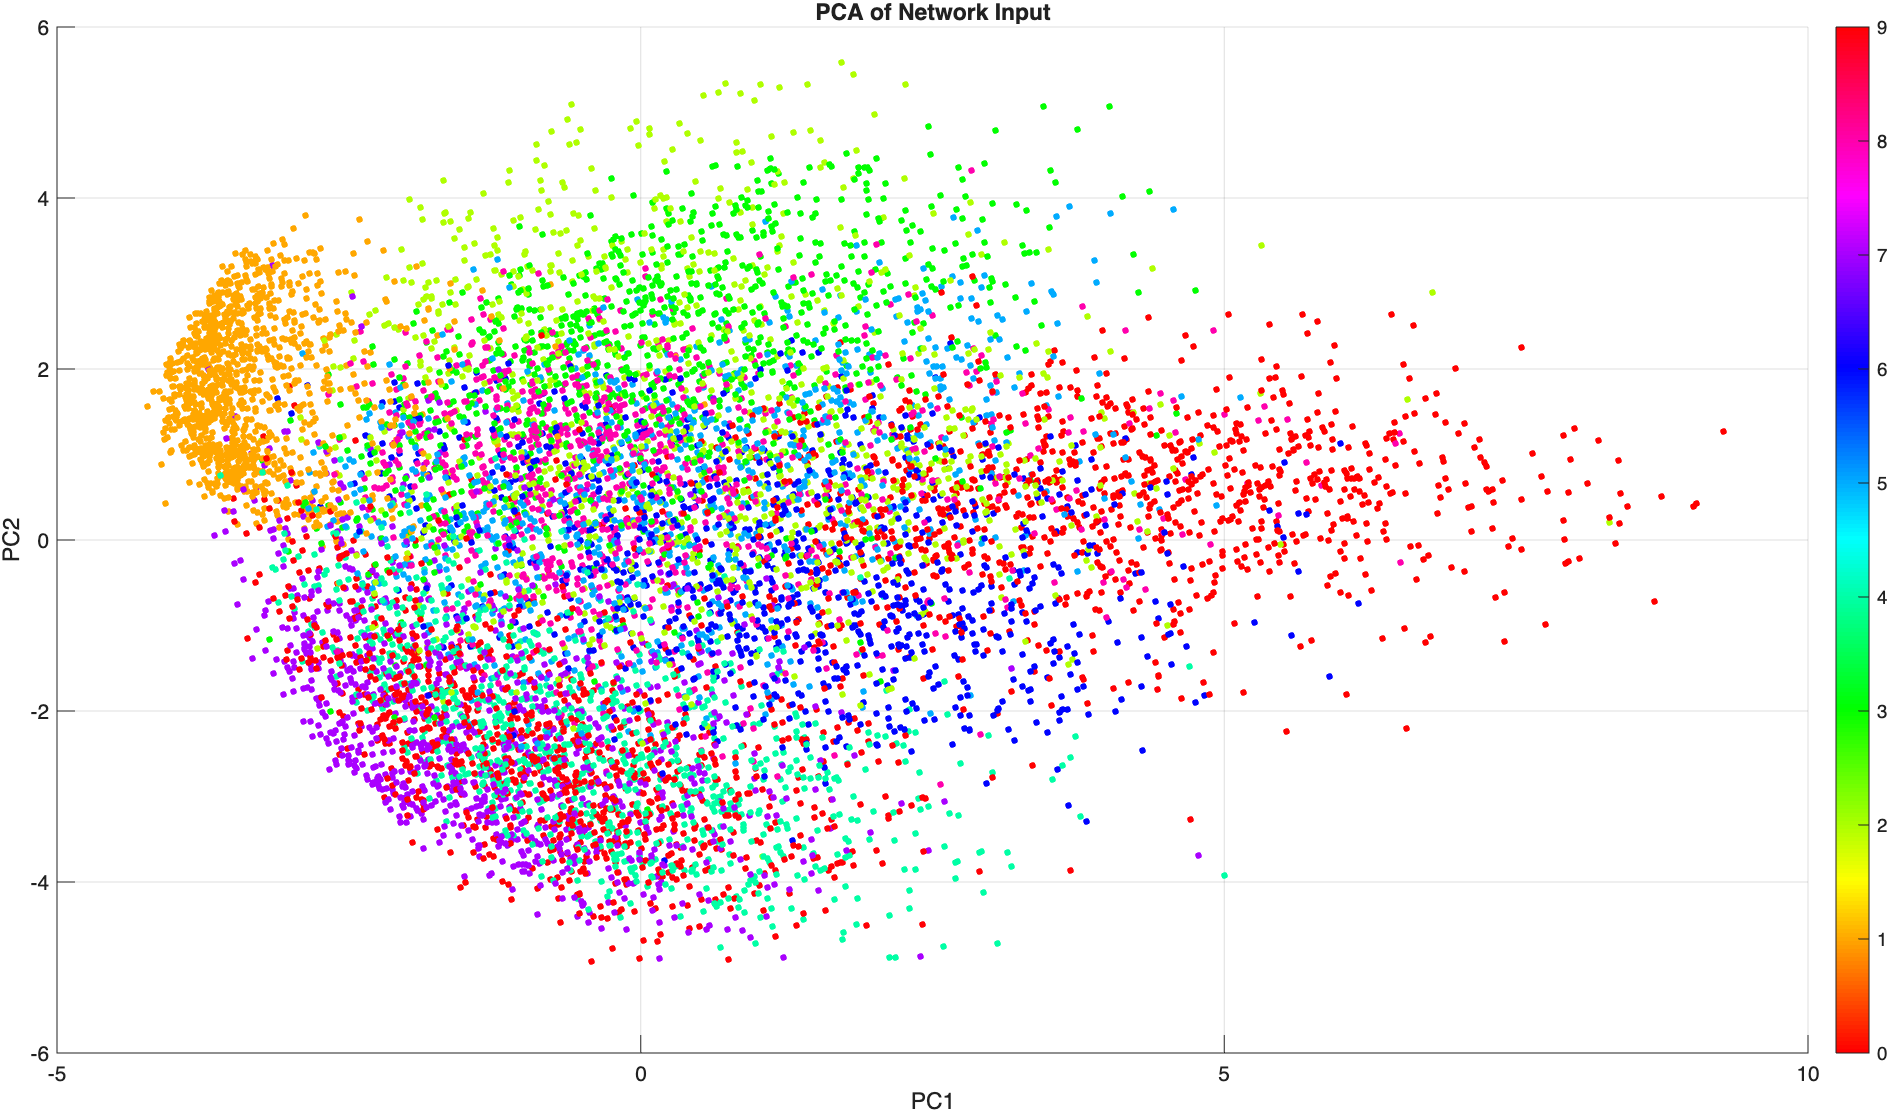
\includegraphics[width=\textwidth]{Figures/PCAInput}
         %\caption{$y=x$}
         \label{fig:y equals x}
     \end{subfigure}
     \hfill
     \begin{subfigure}[b]{0.32\textwidth}
         \centering
         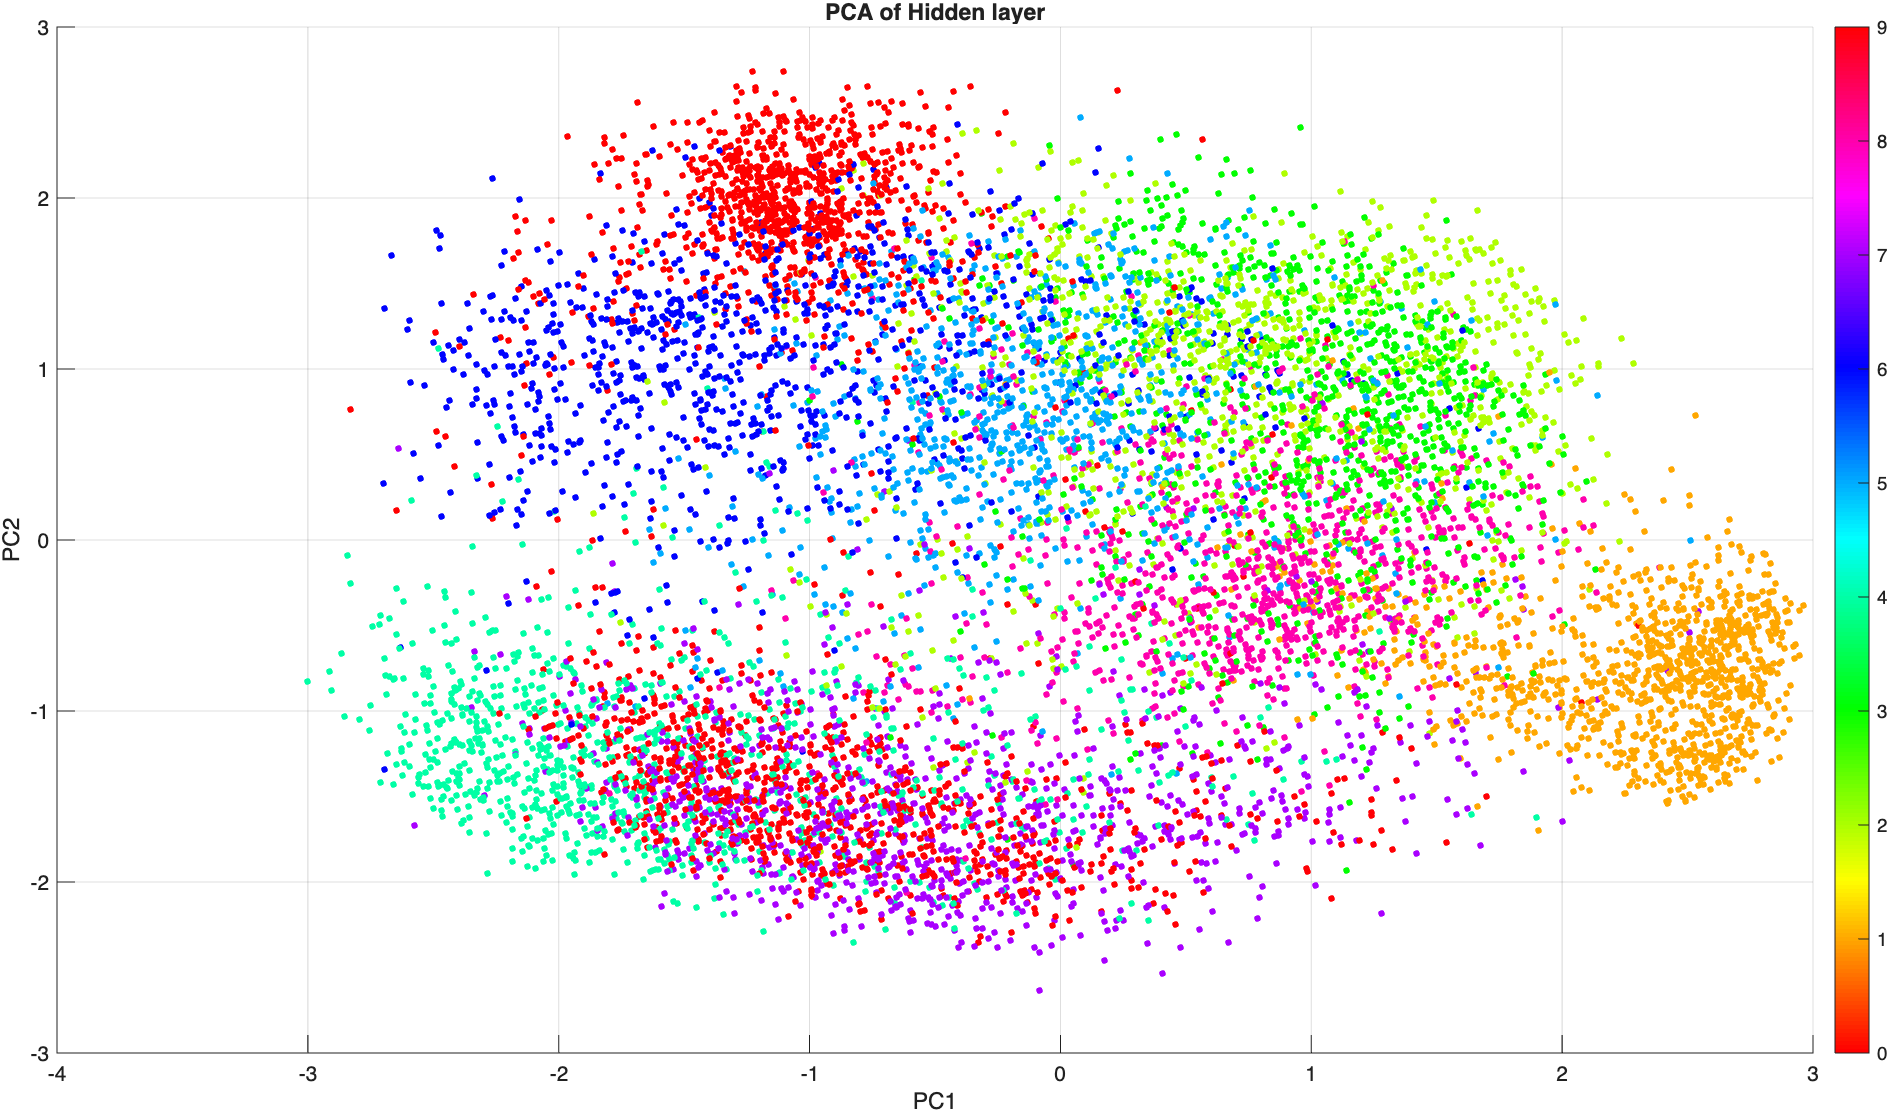
\includegraphics[width=\textwidth]{Figures/PCAHidden}
         %\caption{$y=3\sin x$}
         \label{fig:three sin x}
     \end{subfigure}
     \hfill
     \begin{subfigure}[b]{0.32\textwidth}
         \centering
         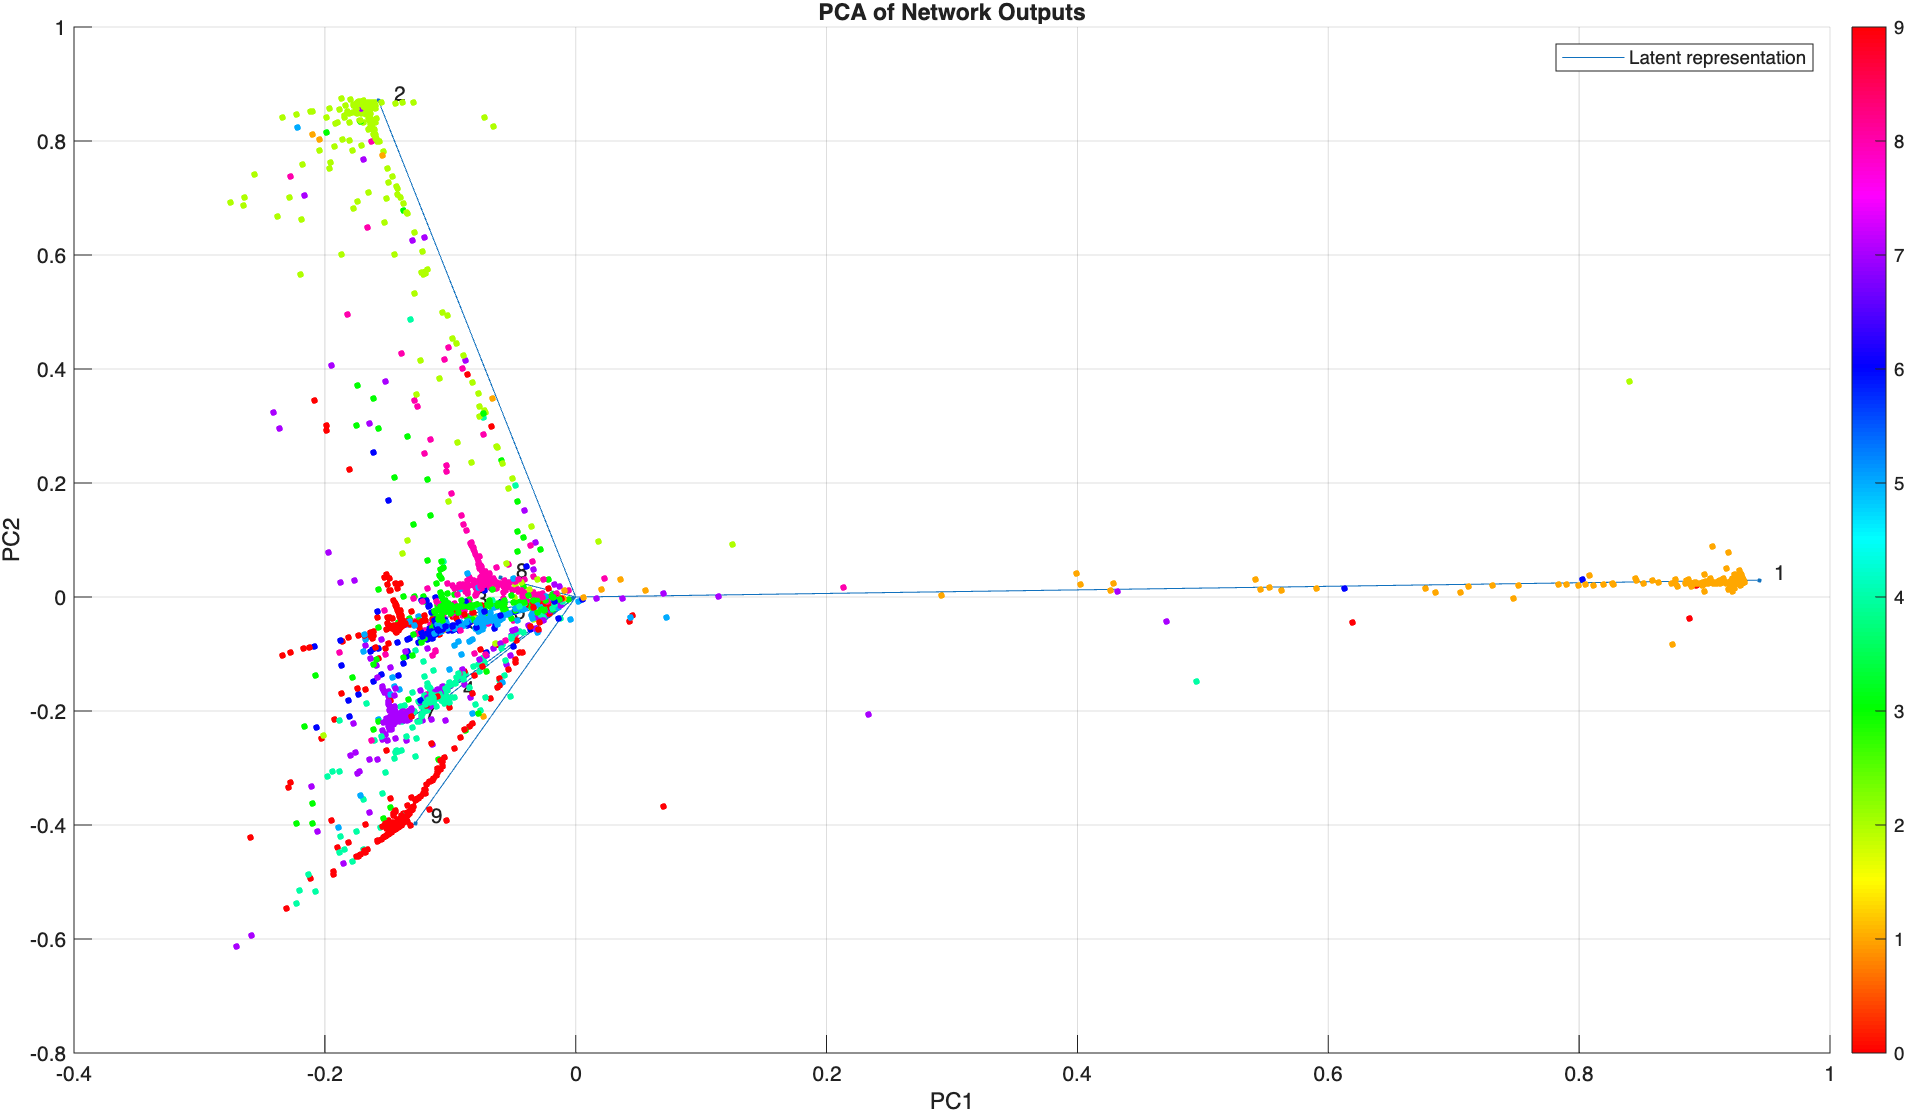
\includegraphics[width=\textwidth]{Figures/PCAOutput.png}
         \label{fig:five over x}
     \end{subfigure}
        \caption{Score plot from the PCA analysis on the input layer (left), the first hidden layer (middle) and the last layer (right) before the classification. The colors correspond to the correct classification. For the second (last) hidden layer, a biplot is provided where the loadings correspond to the models predictions.}
        \label{fig:PCA}
\end{figure}

\section{LLE}
With local linear embedding, we can see in Figure \ref{fig:LLE} that only some digits are separable in the input layer, while on the output layer nearly all classes are spread closely around a single line. In the hidden layer, we can see that the different classes are nearly spread around an interval of a line.  For the amount of neighbors 20 was chosen and the amount of dimensions was set to 6. It might be that the data is not fully local linear and therefore UMAP will obtain better results.
\begin{figure}[h!]
     \centering
     \begin{subfigure}[b]{0.32\textwidth}
         \centering
         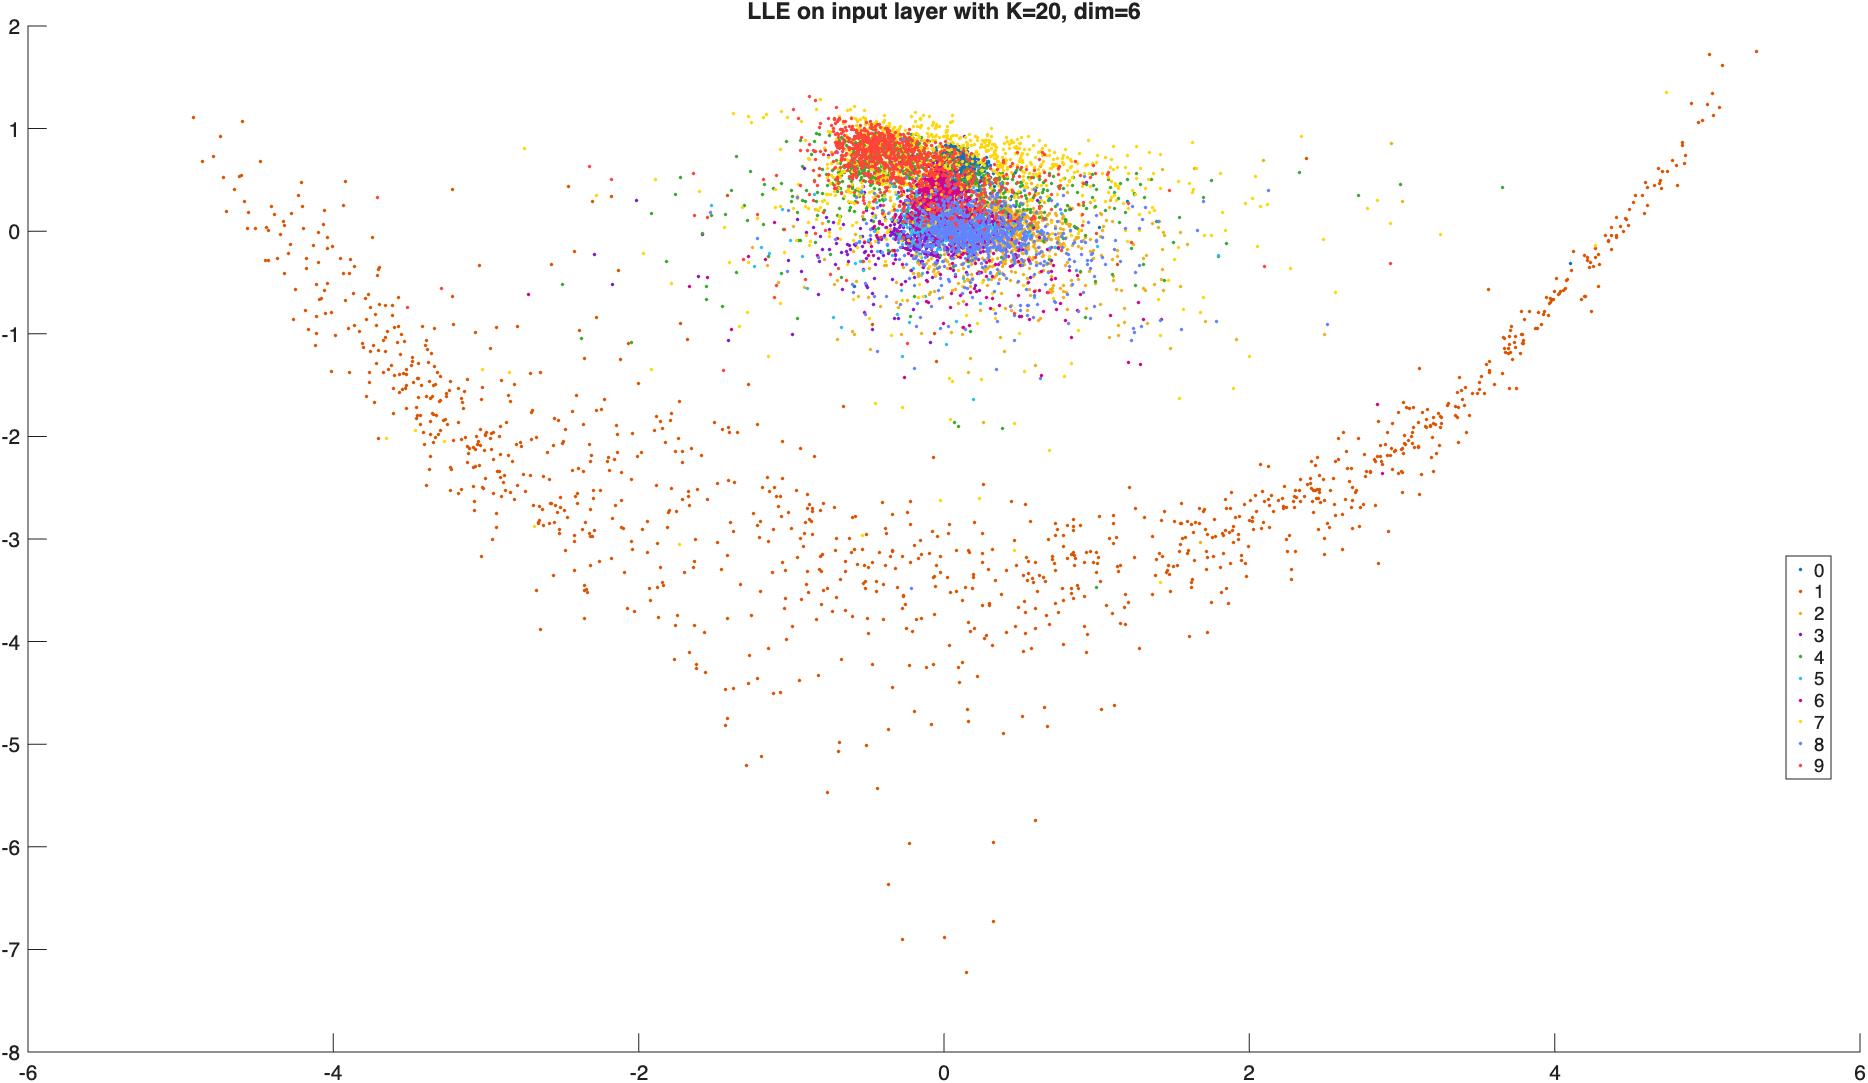
\includegraphics[width=\textwidth]{Figures/LLEInput}
         %\caption{$y=x$}
         \label{fig:y equals x}
     \end{subfigure}
     \hfill
     \begin{subfigure}[b]{0.32\textwidth}
         \centering
         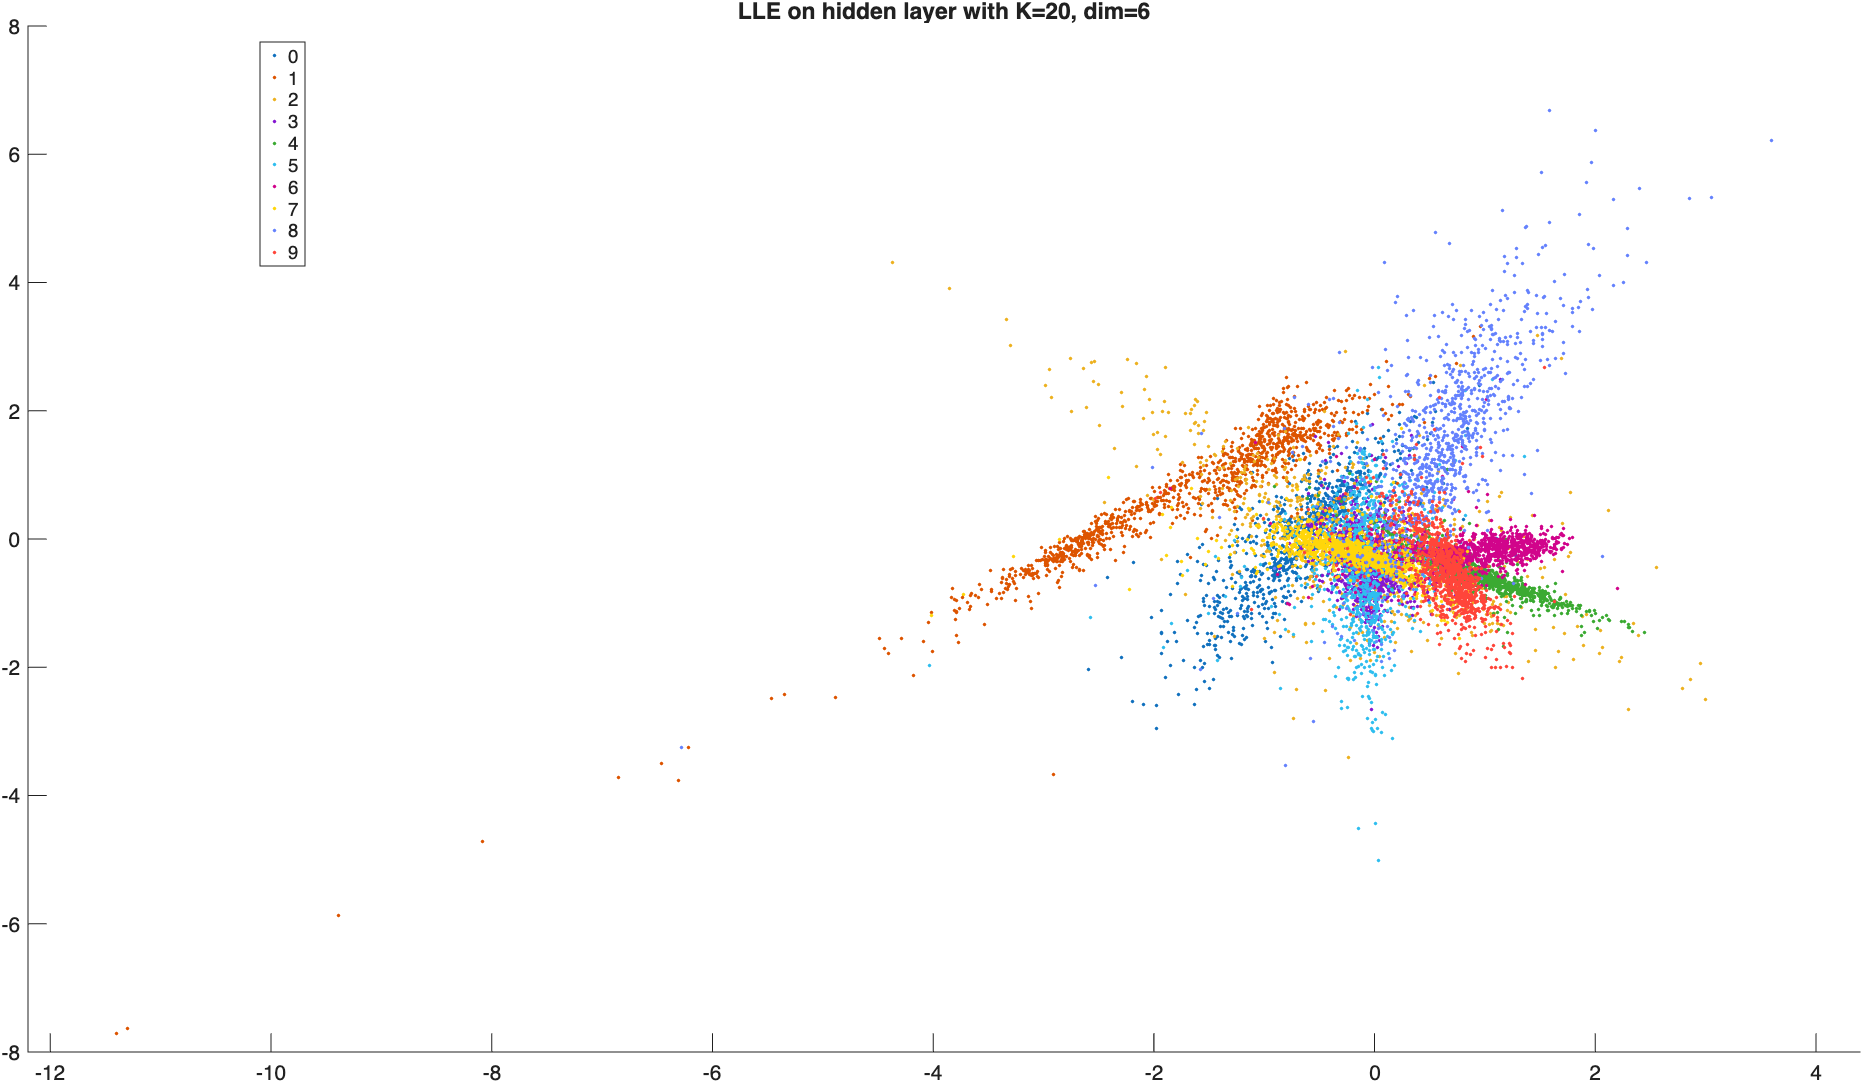
\includegraphics[width=\textwidth]{Figures/LLEHidden}
         %\caption{$y=3\sin x$}
         \label{fig:three sin x}
     \end{subfigure}
     \hfill
     \begin{subfigure}[b]{0.32\textwidth}
         \centering
         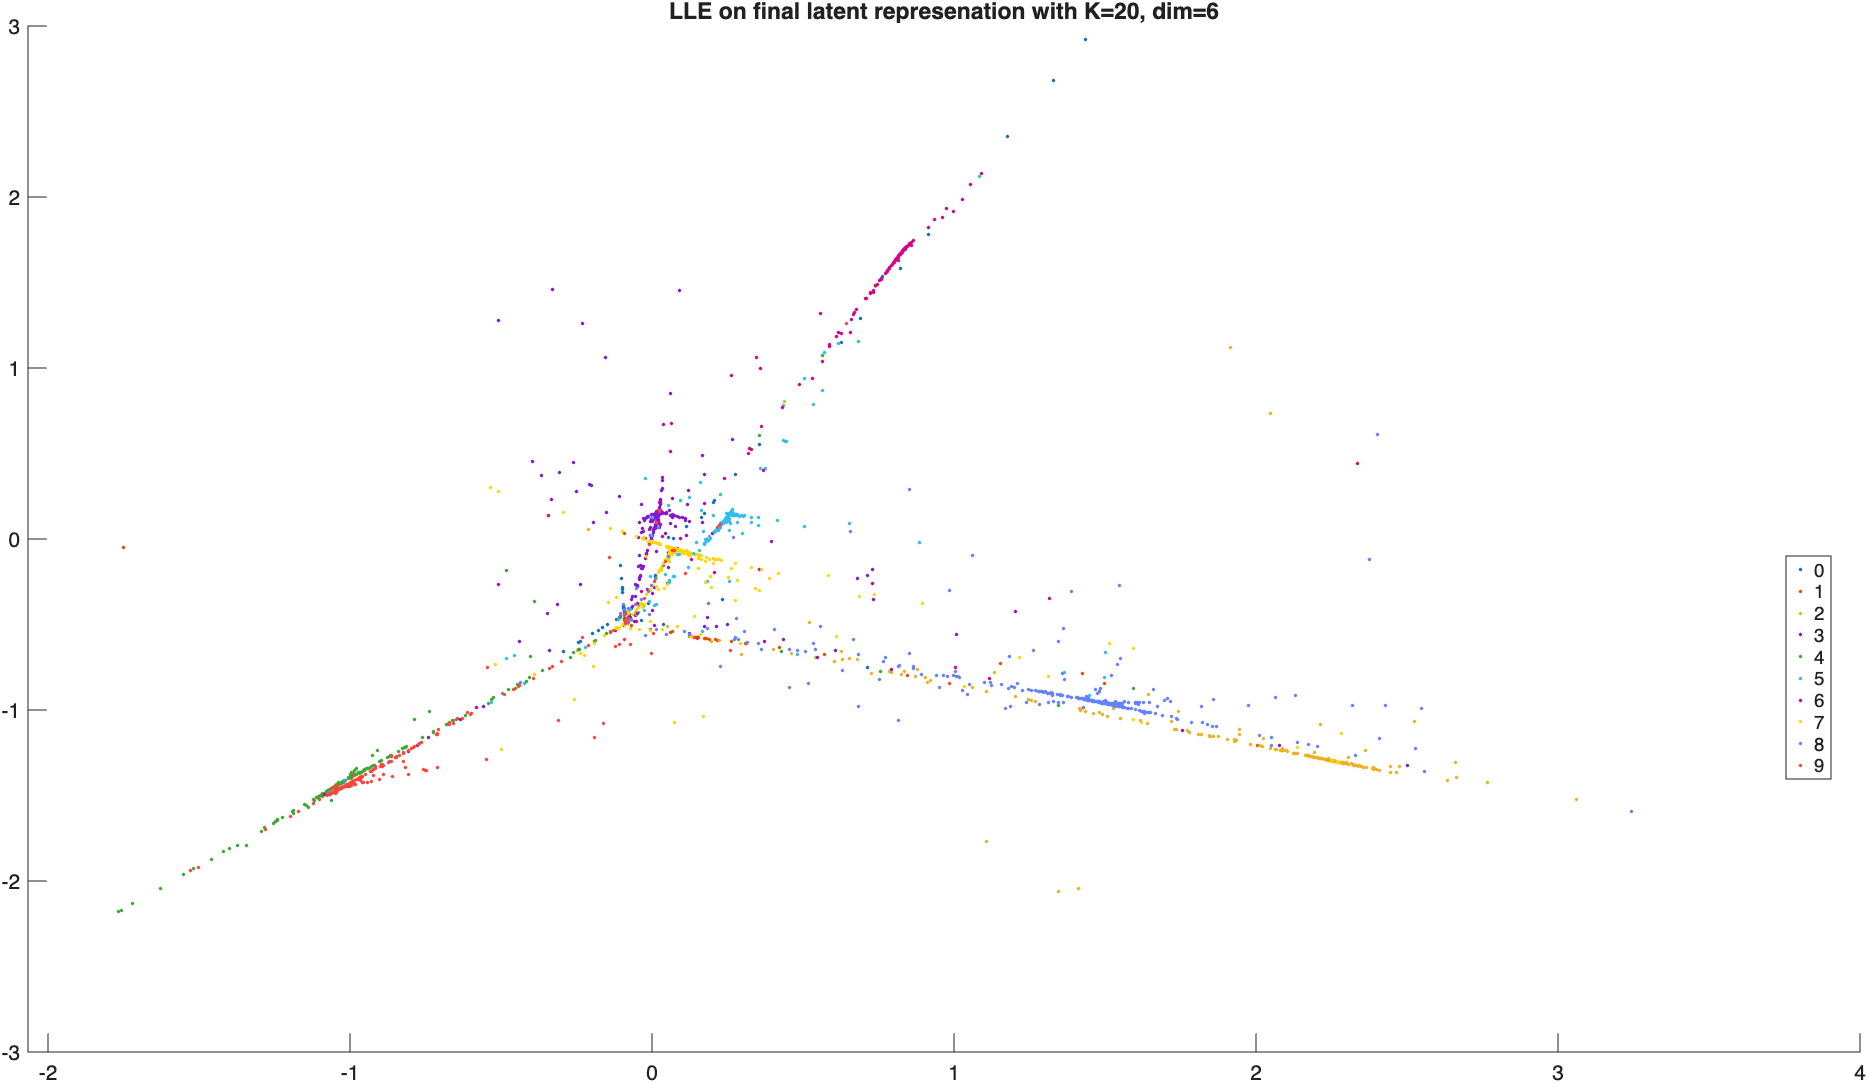
\includegraphics[width=\textwidth]{Figures/LLEOut}
         \label{fig:five over x}
     \end{subfigure}
        \caption{Scatter plot on the two dimensional representation using LLE on the input layer (left), hidden layer (middle) and the second hidden layer (right). The colors correspond to the correct classification. }
        \label{fig:LLE}
\end{figure}
\section{UMAP}
We can see in Figure \ref{fig:UMAP} that in this representation, all the groups are clearly distinct and separable, except for some outliers which are probably wrong classifications by the model assuming the dataset is flawless.  This suggests that the neural network is in fact able to separate the digits up to some accuracy. 

\begin{figure}[h!]
     \centering
     \begin{subfigure}[b]{0.32\textwidth}
         \centering
         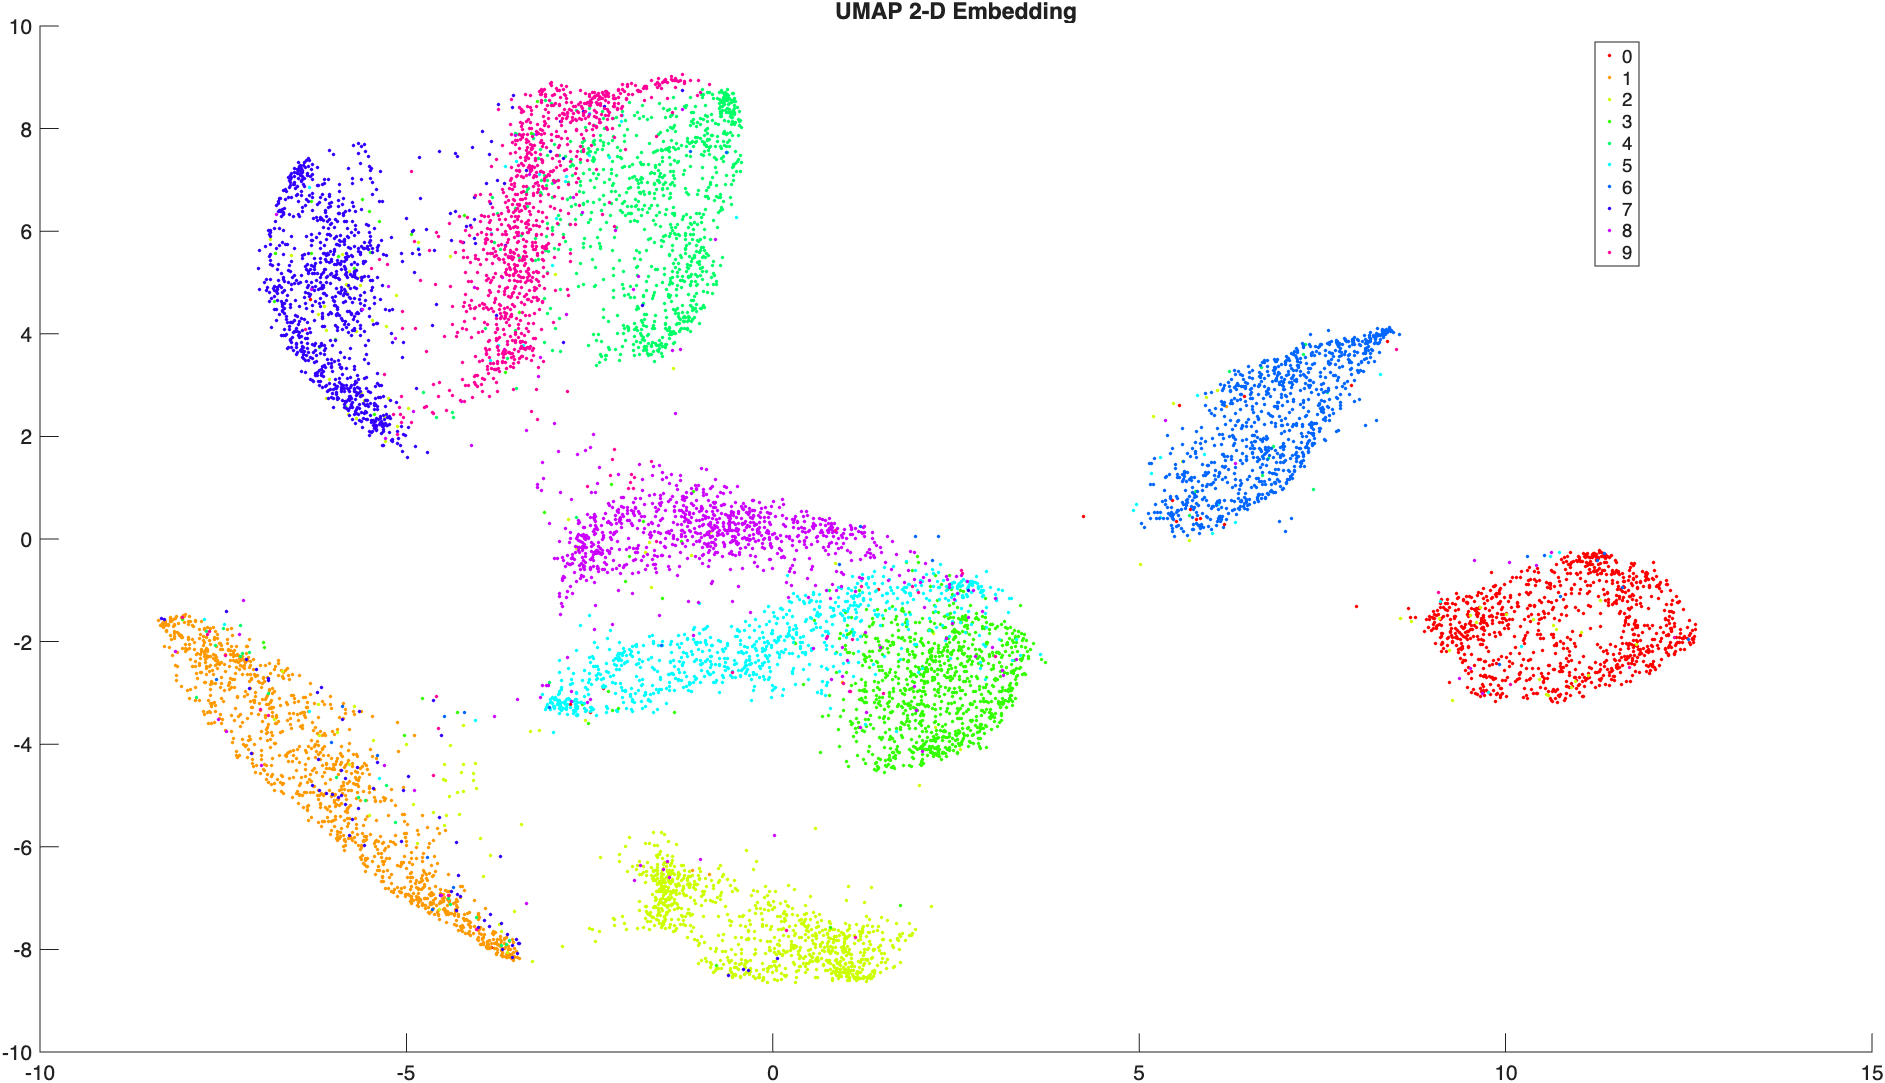
\includegraphics[width=\textwidth]{Figures/UMapInput}
         %\caption{$y=x$}
         \label{fig:y equals x}
     \end{subfigure}
     \hfill
     \begin{subfigure}[b]{0.32\textwidth}
         \centering
         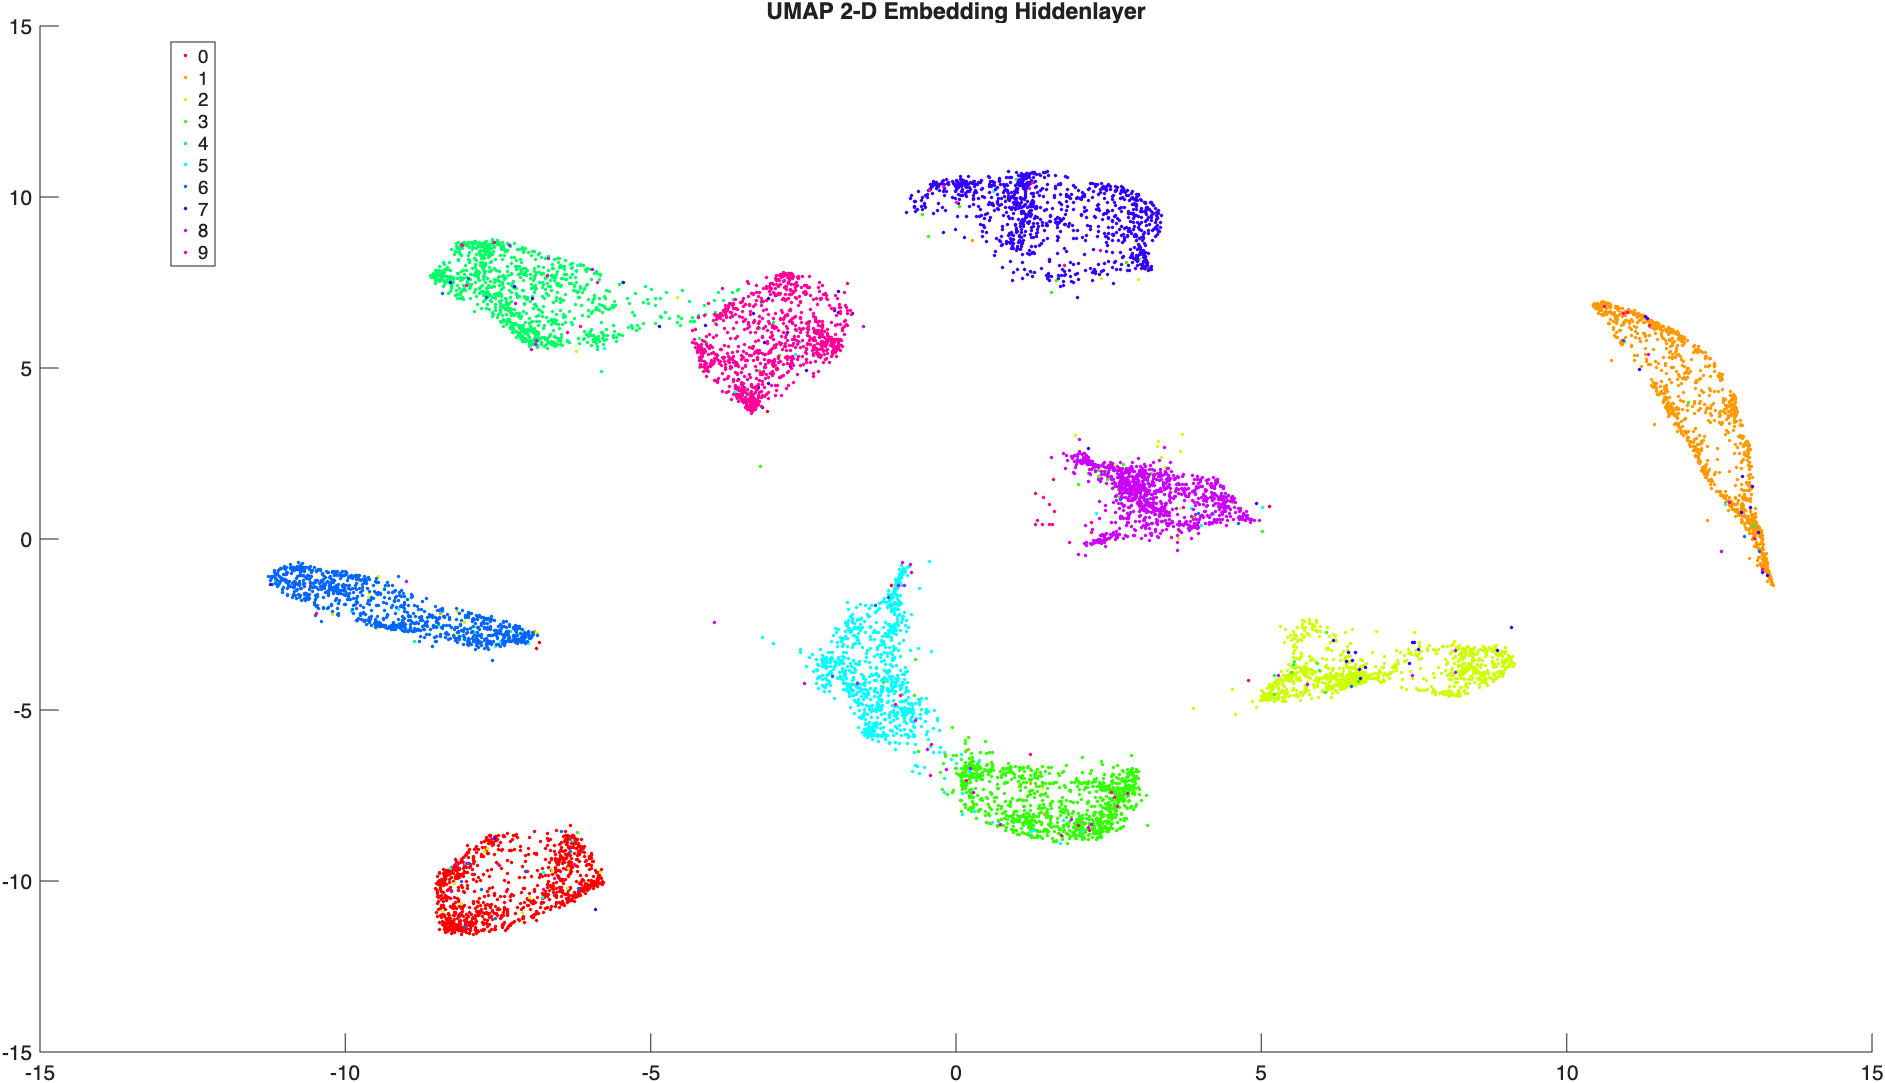
\includegraphics[width=\textwidth]{Figures/UMapHidden}
         %\caption{$y=3\sin x$}
         \label{fig:three sin x}
     \end{subfigure}
     \hfill
     \begin{subfigure}[b]{0.32\textwidth}
         \centering
         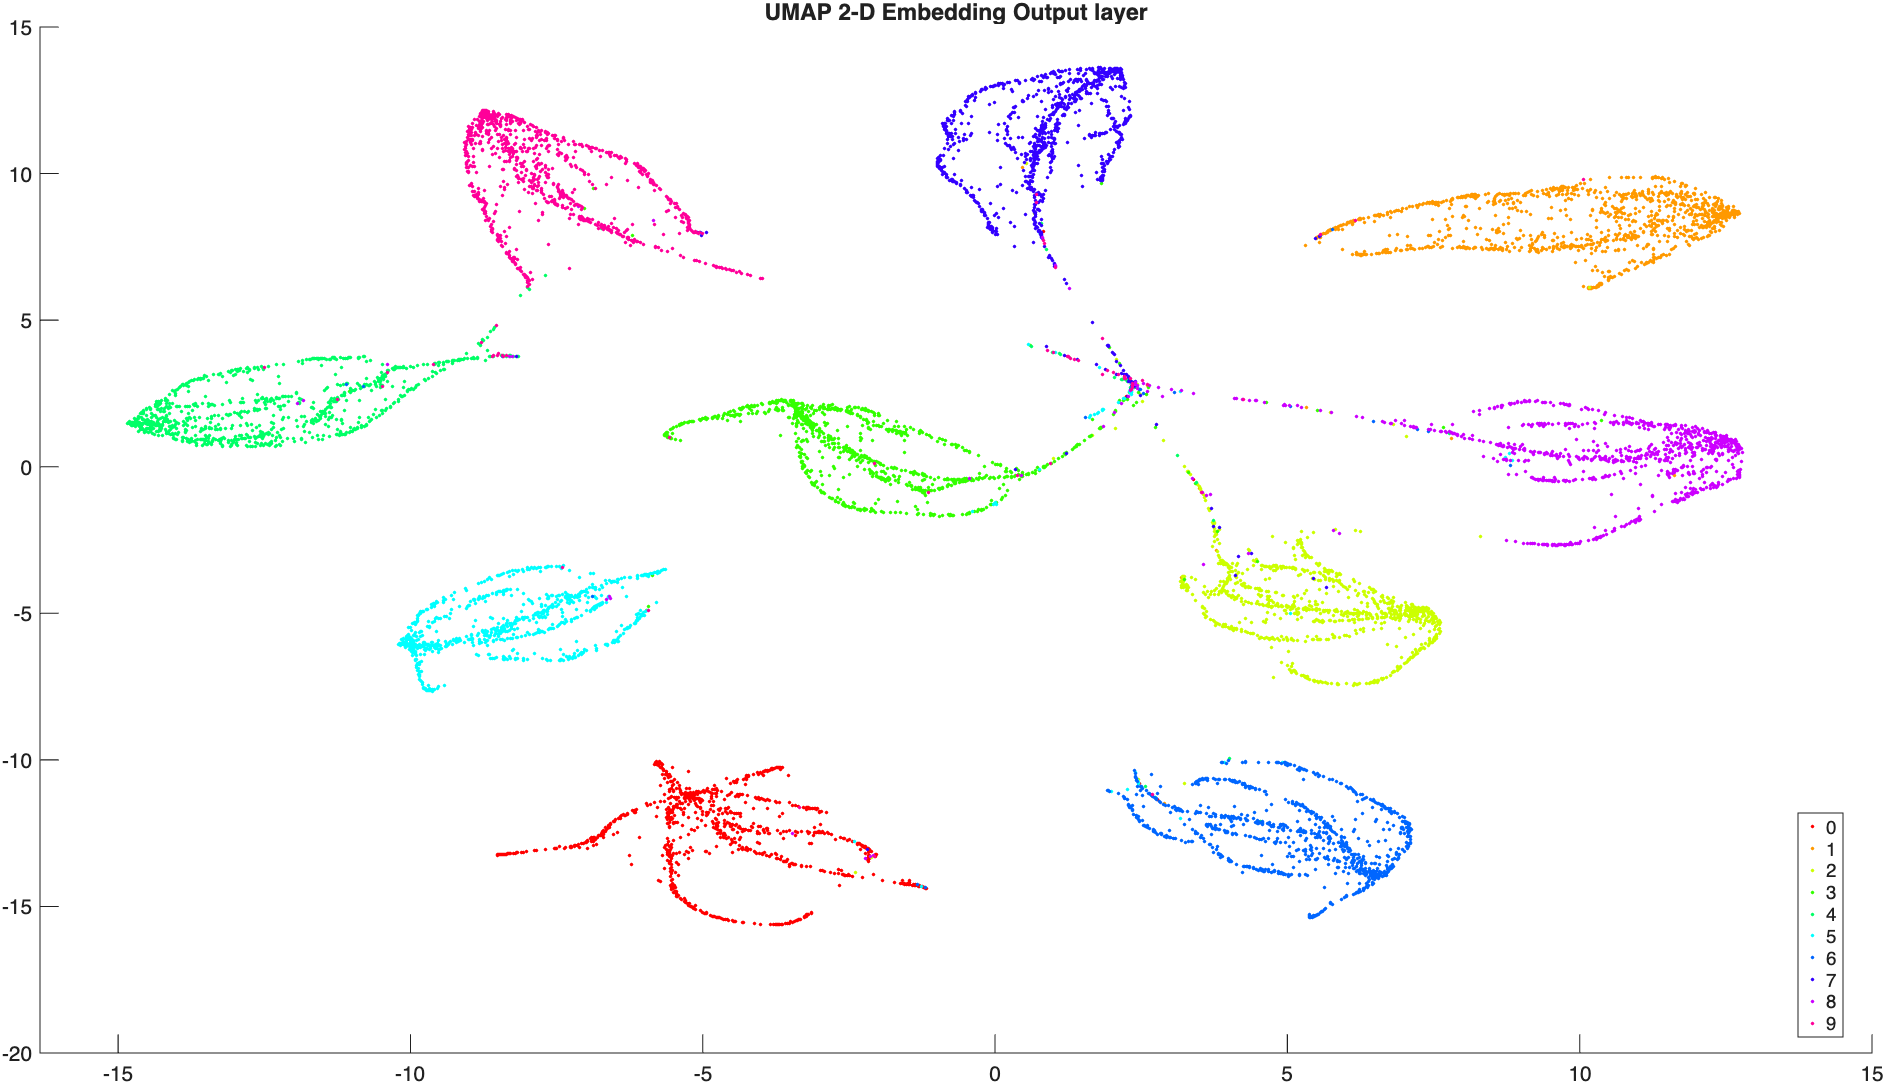
\includegraphics[width=\textwidth]{Figures/UMAPOutput}
         \label{fig:five over x}
     \end{subfigure}
        \caption{UMAP two dimensional embedding on the input layer (left), hidden layer (middle) and the second hidden layer (right). The colors correspond to the correct classification. }
        \label{fig:UMAP}
\end{figure}

The optimal hyper-parameters were found by iterating through some possible hyper-parameters, an embedding density of 1 and 15 neighbors seems to capture the groups well as we can see in Figure \ref{fig:UMAPComp}.

\begin{figure}[h!]
\centering
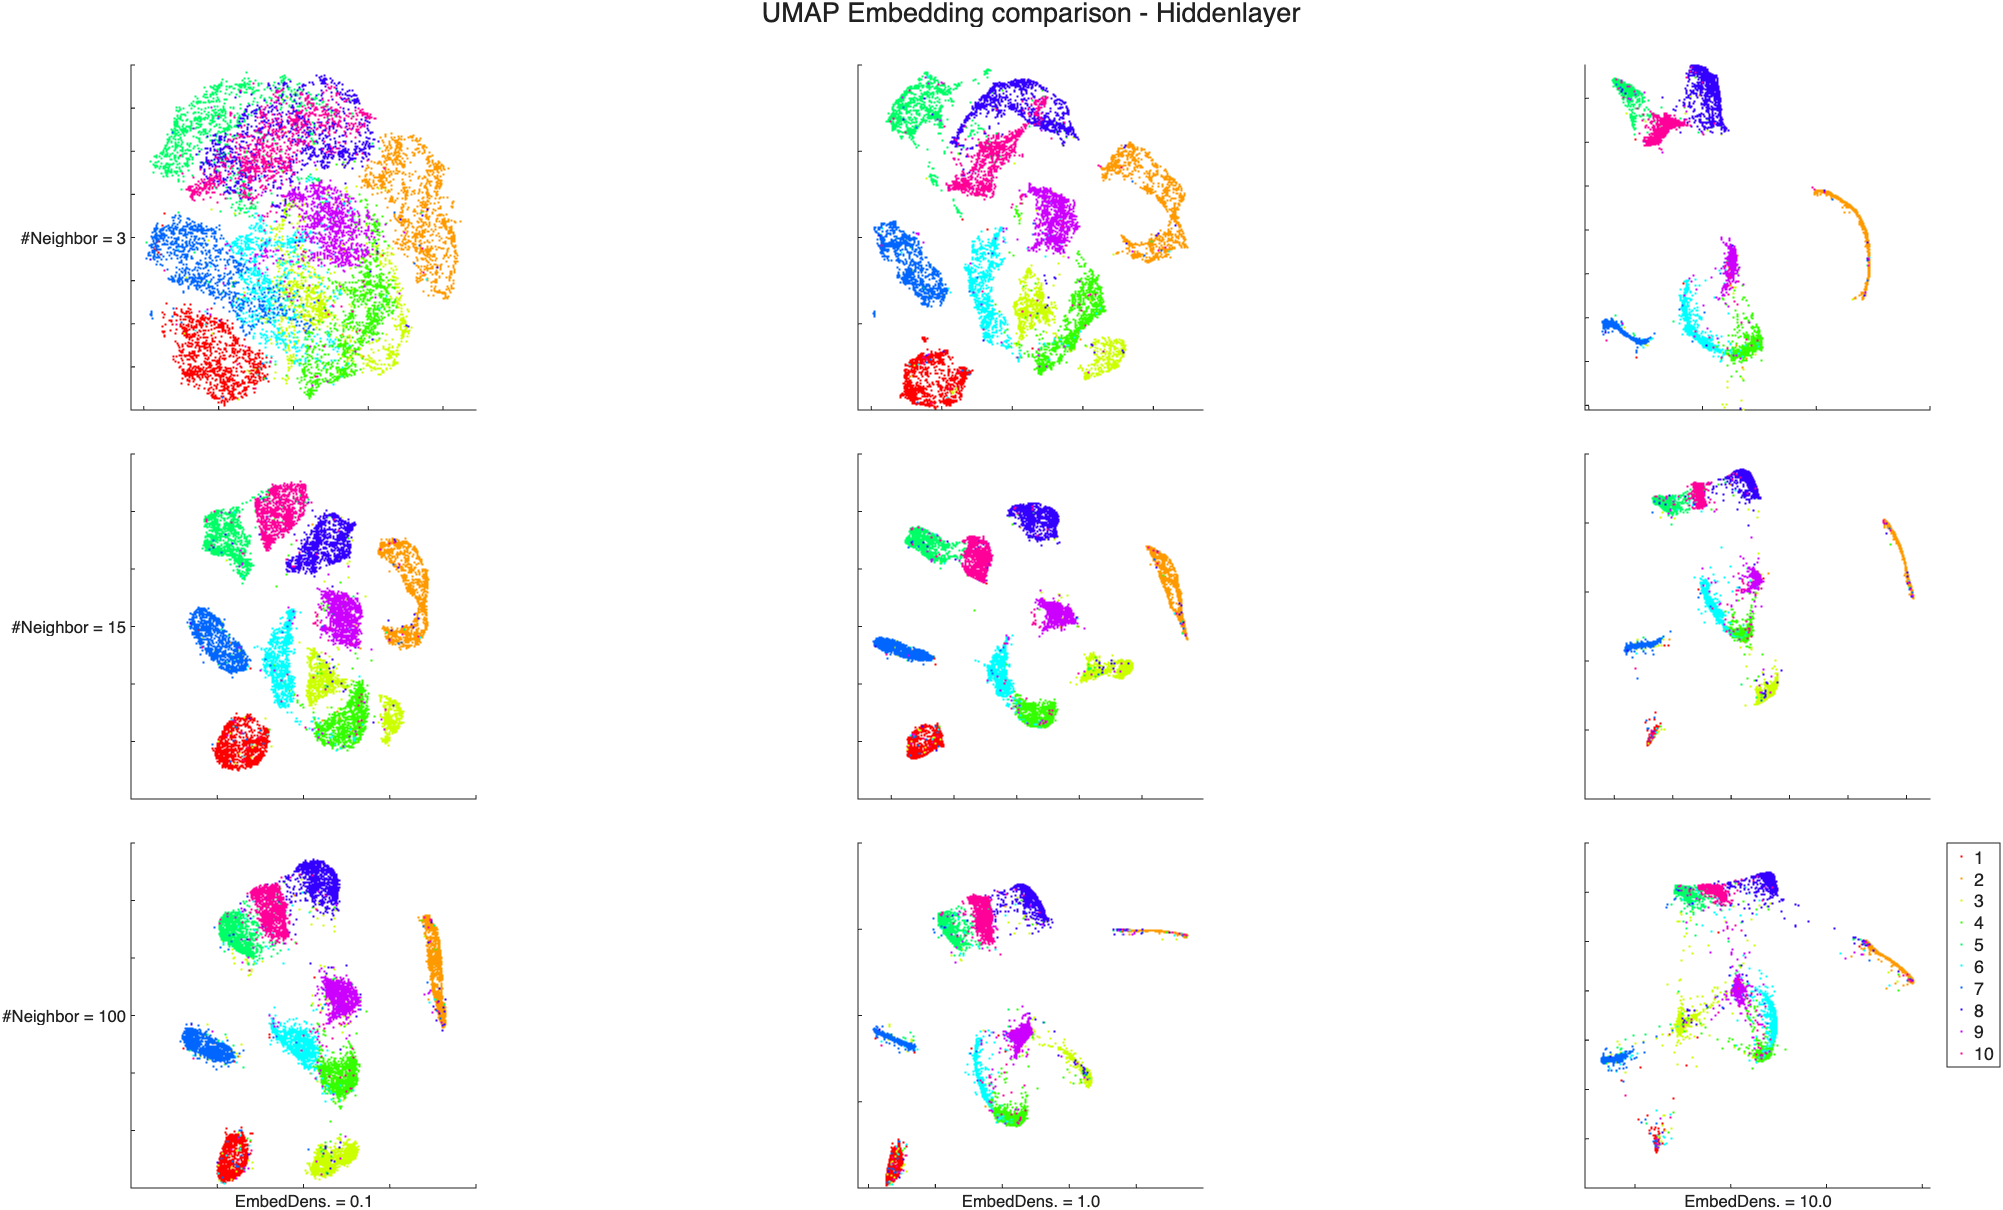
\includegraphics[width=\textwidth]{Figures/UMAPComparisonH}
\caption{Comparison for different densities and amounts of neighbors. UMAP two dimensional embedding on the hidden layer. The colors correspond to the correct classification. }
\label{fig:UMAPComp}
\end{figure}

\section{SOM}
Unfortunately, due to the ten different digits, it seems impractical to use SOM to represent this fact for analyzing a neural network. We can see in the left of Figure \ref{fig:SOM} that no interpretability can result from this. There might exist other parameters which allow improvements for this. For a smaller subset of digits, we can see some improvements as in the right of \ref{fig:SOM}
\begin{figure}[h!]
     \centering
     \begin{subfigure}[b]{0.48\textwidth}
         \centering
         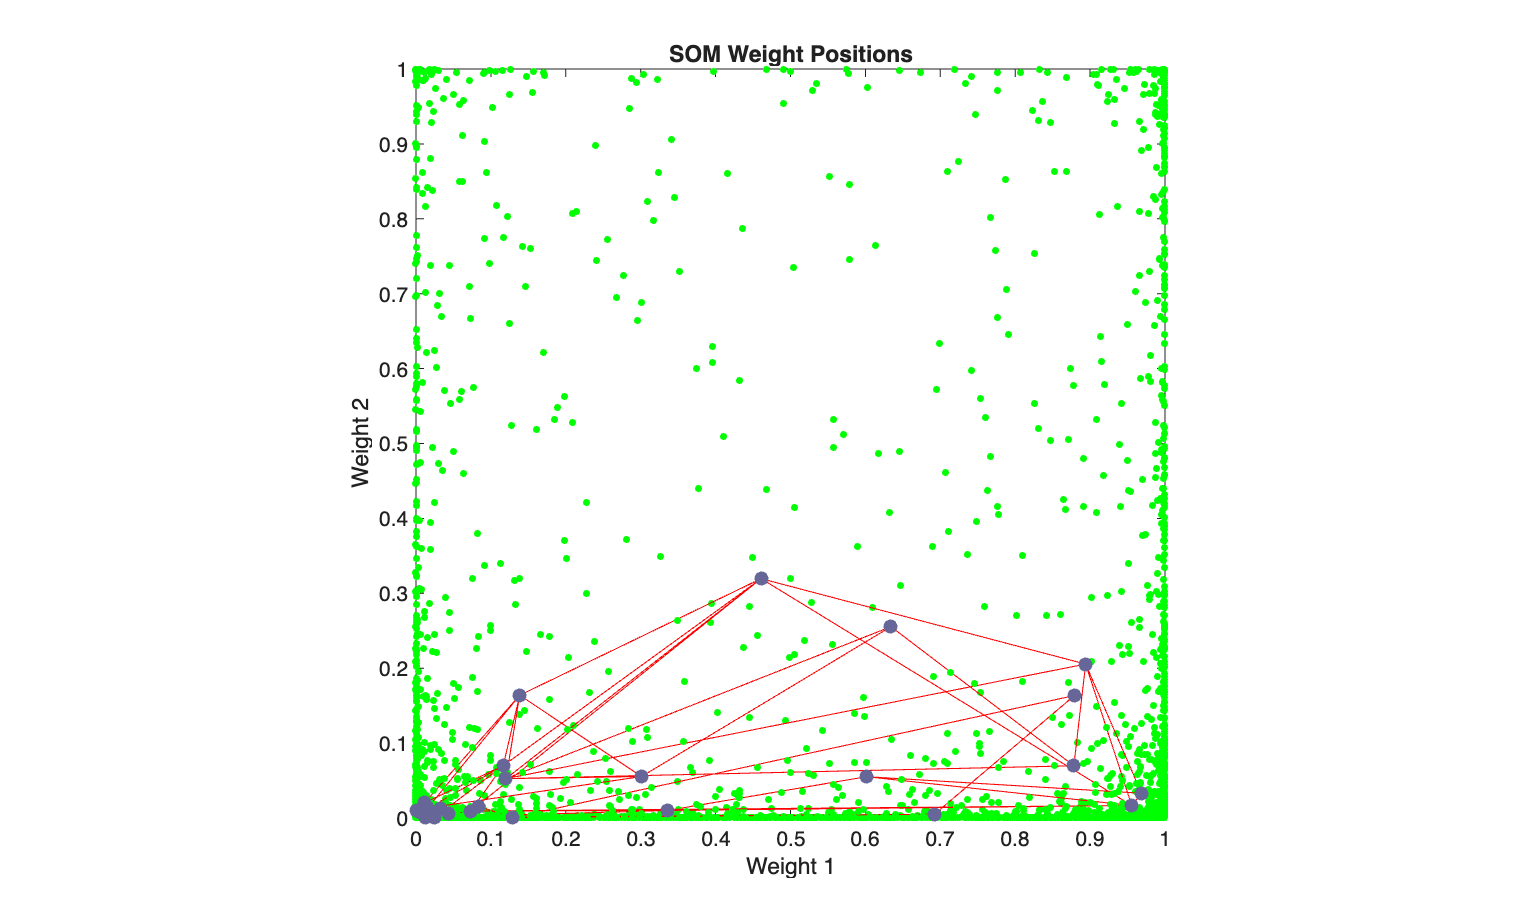
\includegraphics[width=\textwidth]{Figures/SOMHiddenWeight}
         %\caption{$y=x$}
         \label{fig:y equals x}
     \end{subfigure}
     \hfill
     \begin{subfigure}[b]{0.48\textwidth}
         \centering
         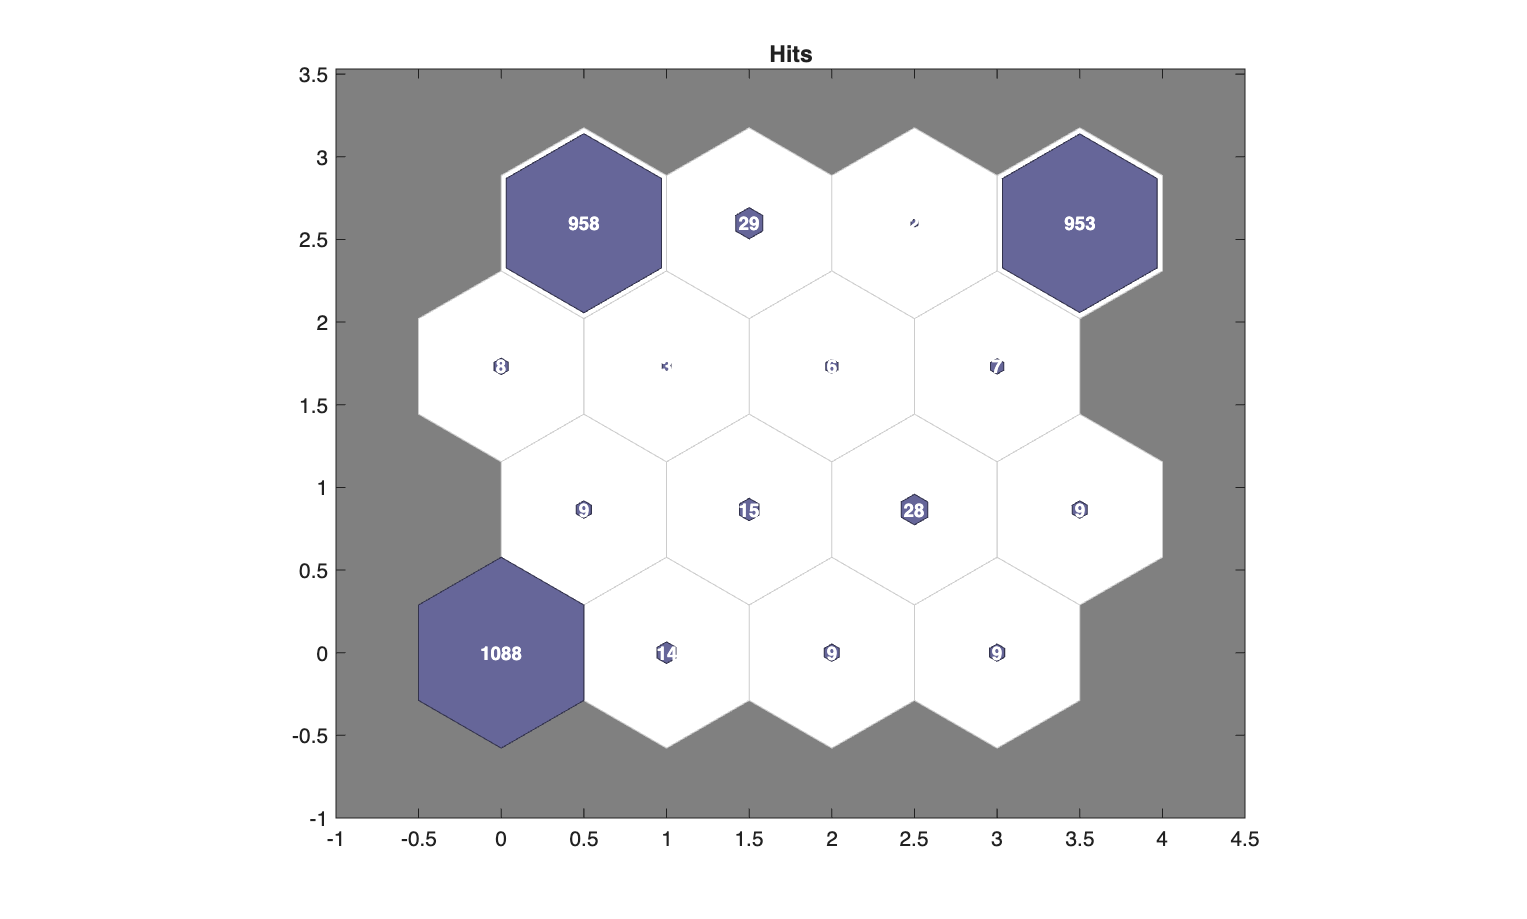
\includegraphics[width=\textwidth]{Figures/SOMHitsOutputreduced}
         %\caption{$y=3\sin x$}
         \label{fig:three sin x}
     \end{subfigure}
   
        \caption{SOM analysis: Weight positions with dimensionality of 5 x  5 (left), number of hits of individual neurons of the output layer dimensions for digits 0,1,2 only with dimensions 2x2(right) }
        \label{fig:SOM}
\end{figure}
\section{No training}
If the neural network is not trained, then the separation should fail in particular for last hidden layer, which is indeed what we can observe in Figure \ref{fig:UMAPuntrained}. Note that the first hidden layer lets us still separate most of the digits, this is due to the fact that still most of the features are passed from the first layer even if the model is not trained this data is enough to disseminate most of the digits. 
\begin{figure}[h!]
     \centering
     \begin{subfigure}[b]{0.48\textwidth}
         \centering
         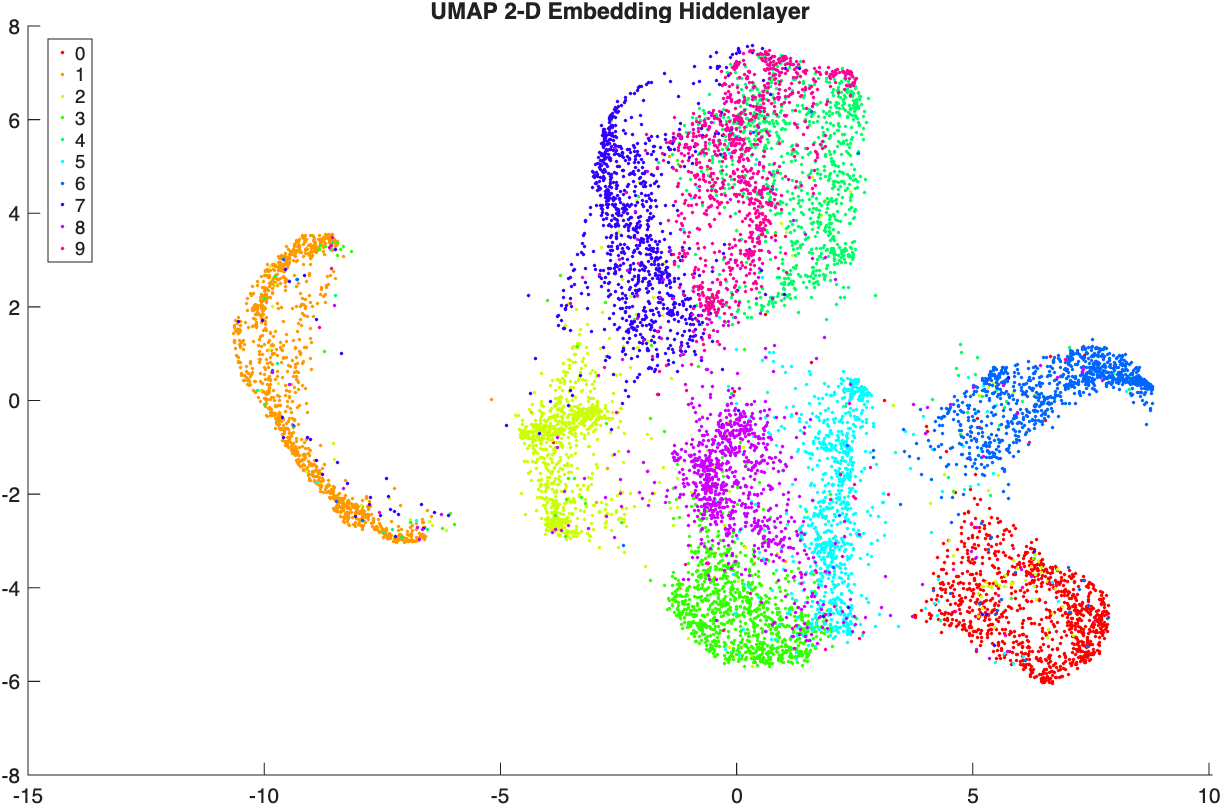
\includegraphics[width=\textwidth]{Figures/UntrainedUMAPHidden}
         %\caption{$y=x$}
         \label{fig:y equals x}
     \end{subfigure}
     \hfill
     \begin{subfigure}[b]{0.48\textwidth}
         \centering
         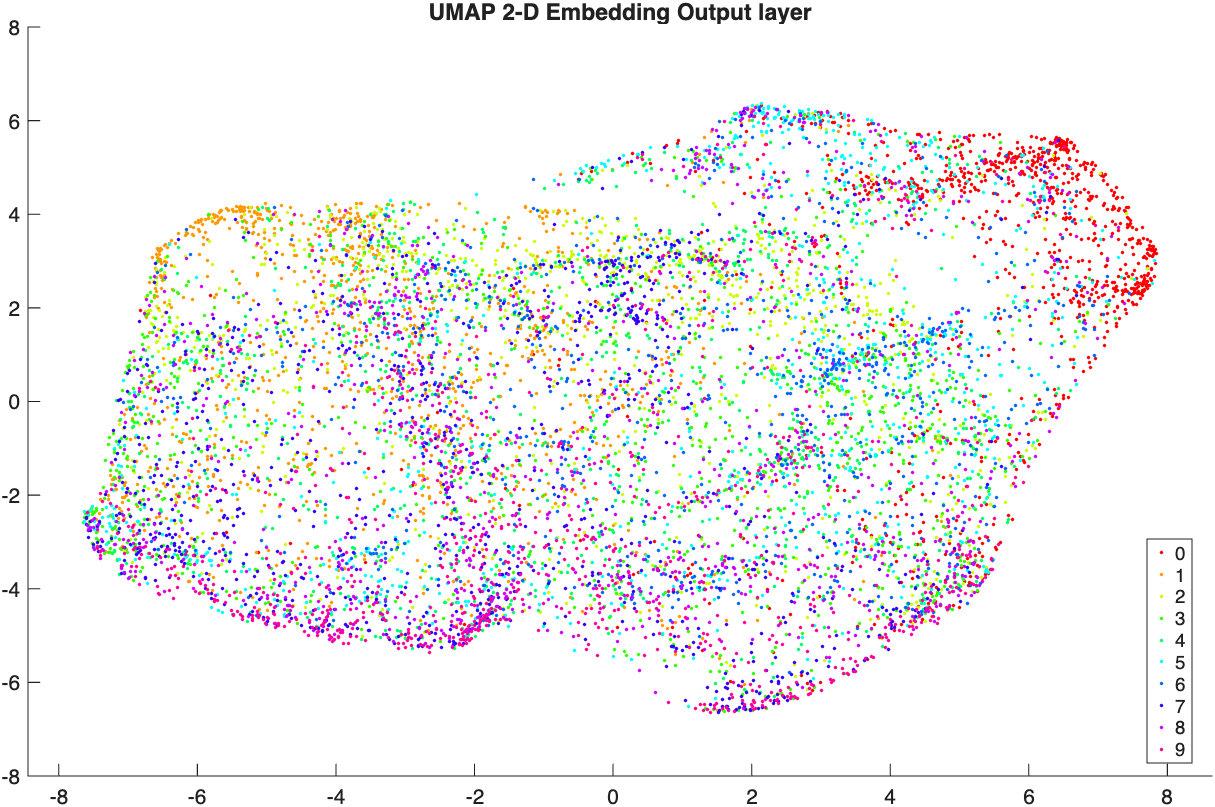
\includegraphics[width=\textwidth]{Figures/UntrainedUMAPOut}
         %\caption{$y=3\sin x$}
         \label{fig:three sin x}
     \end{subfigure}
   
        \caption{UMAP representation of an untrained model of the first hidden layer(left) and the second hidden layer (right) . The colors correspond to the correct classification. }
        \label{fig:UMAPuntrained}
\end{figure}
\section{Conclusions}
For the digit dataset, the use of methods representing the data in high dimensions is not advantageous, so we can observe that UMAP embedding allows for the best visual separability and also it represents the fact of the training of the model, as we saw that untrained models do not lead to separtion. PCA and LLE obtain decent results, but would also profit from a representation in more dimensions. Furthermore for SOM no adequate parameters were found, due to the presence of ten categories, reducing this allows for better interpretability in particular on the precise neurons involved. 
% ======== END OF MAIN TEXT ========
%\nocite{*} % if this line is present, everything is inserted in the bibliography file will be inserted at the end. If removed, only the entry actually cited will be displayed
\FloatBarrier
\bibliographystyle{IEEEtran}
% argument is your BibTeX string definitions and bibliography database(s)
\begin{thebibliography}{9}
\bibitem{script}
Johannes Langelaar (2026). MNIST neural network training and testing (\href{}{https://se.mathworks.com/matlabcentral/fileexchange/73010-mnist-neural-network-training-and-testing}), MATLAB Central File Exchange. Retrieved November 6, 2026.


\end{thebibliography}

%\clearpage
%\appendix


\end{document}
